\documentclass[../../../../main.tex]{subfiles}
\begin{document}

\begin{flushright}
\footnotesize\textit{【自動文字起こし・要確認】}
\end{flushright}

\noindent
[\textbf{解}]
\begin{enumerate}
    \item[(1)] $n$ 個の頂点の中から3つ選べば三角形が1つ対応するので、
    \[
    _n\mathrm{C}_3 = \frac{1}{6}n(n-1)(n-2)
    \]

    \item[(2)] (1)から、鈍角三角形、直角三角形のものをのぞけばよい。

    \begin{enumerate}
        \item[$1^\circ$] $n = 2k\ (k \in \mathbb{N}_{\ge 2})$ の時\\
        1つの頂点を $A_1$ とする。$A_1 A_{k+1}$ が外接円の直径だから、鈍角をつくるには右図の分領域から2点を考えればよく、
        \[
        \begin{cases}
        k \ge 3 \text{のとき} & _{k-1}\mathrm{C}_2 \text{通り} \\
        k \le 2 \text{の時} & 0 \text{通り}
        \end{cases}
        \]
        1つの頂点が他にある場合と重複を考えて、
        \[
        \begin{cases}
        k \ge 3 \text{の時} & 2k \cdot _{k-1}\mathrm{C}_2 / 2 = k(k-1)(k-2) \text{通り} \\
        k \le 2 \text{の時} & 0 \text{通り}
        \end{cases}
        \]

        \begin{center}
        \begin{tikzpicture}[scale=1.2]
            \draw (0,0) circle (1.2);
            \fill (0,1.2) circle (1.5pt) node[above]{$A_1$};
            \fill (0,-1.2) circle (1.5pt) node[below]{$A_{k+1}$};
            \draw[dashed] (0,1.2) -- (0,-1.2);
            \draw[thick] (0.1,1.1) arc (80:-80:1.1);
            \draw[thick] (-0.1,1.1) arc (100:260:1.1);
            \node at (0.5,0.5) {$2\text{つ}$};
        \end{tikzpicture}
        \end{center}

        一方、直角三角形は1つの直径となる辺に対し、のこり1つの辺のえらび方が $2k-2$ 通りあるから、
        \[
        k(2k-2) \text{通り}
        \]

        \item[$2^\circ$] $n = 2k-1$ の時\\
        1°と同様に考える。1つの頂点を $A_1$ に固定した時、鈍角三角形は
        \[
        \begin{cases}
        k \ge 3 \text{のとき} & _{k-1}\mathrm{C}_2 \text{通り} \\
        k \le 2 \text{の時} & 0 \text{通り}
        \end{cases}
        \]
        だから、あわせて
        \[
        \begin{cases}
        k \ge 3 \text{の時} & (2k-1) \cdot _{k-1}\mathrm{C}_2 \text{通り} \\
        k = 2 \text{の時} & 0 \text{通り}
        \end{cases}
        \]
        直角三角形は存在しない。

        \begin{center}
        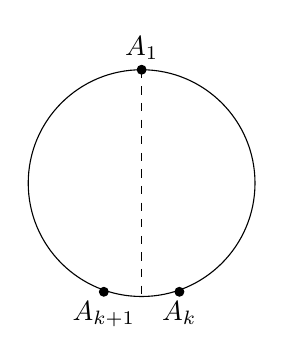
\begin{tikzpicture}[scale=1.2]
            \draw (0,0) circle (1.2);
            \fill (0,1.2) circle (1.5pt) node[above]{$A_1$};
            \fill (-0.4,-1.15) circle (1.5pt) node[below]{$A_{k+1}$};
            \fill (0.4,-1.15) circle (1.5pt) node[below]{$A_k$};
            \draw[dashed] (0,1.2) -- (0,-1.2);
        \end{tikzpicture}
        \end{center}
    \end{enumerate}

    以上から、求める数は $n=3$ の時 1、$n=4$ の時 0 で、$n \ge 5$ の時
    \[
    n \in \text{even の時}: \quad \frac{1}{6}n(n-1)(n-2) - \frac{n}{2}\left(\frac{n}{2}-1\right)\left(\frac{n}{2}-2\right) - \frac{n}{2}(n-2) = \frac{1}{24}n(n-2)(n-4)
    \]
    \[
    n \in \text{odd の時}: \quad \frac{1}{6}n(n-1)(n-2) - \frac{1}{2}n\left(\frac{n-1}{2}\right)\left(\frac{n-3}{2}\right) = \frac{1}{24}n(n+1)(n-1)
    \]
    これらは $n=3, 4$ でも成立するから
    \[
    \begin{cases}
    n \in \text{odd} & \frac{1}{24}n(n+1)(n-1) \\
    n \in \text{even} & \frac{1}{24}n(n-2)(n-4)
    \end{cases}
    \]
    である。
\end{enumerate}

\end{document}
